
\subsection{Introduction to convex optimization problems}
General form: Consider the functions $F_i(x), h_i(x): \reals^n\rightarrow \reals$.
\begin{align*}
\min_{x\in \reals^n} \quad &F_0(x) \quad \text{"objective function"}\\
s.t. \quad &F_i(x) \leq 0, i = 1...m \quad\text{inequality constraints}\\
&h_i(x) =0,i =1...p \quad \text{equality constraints}
\end{align*}


Feasible set for this question:
$$\mathcal{C} = \{x\vert F_i(x) \leq 0,i=1...m,h_i(x) = 0,i = 1...p \}$$


Optimal value: $p^* = \inf_{x\in \mathcal{C}}F_0(x)$. Note that it could be $\infty$, and also could be empty.

Optimal points: $\{x\in \mathcal{C}\vert F_0(x) = p^* \}$. Note that it could be empty, and also could be not unique.



\begin{example}
Consider the optimization problem:
\begin{align*}
\min_x \quad &\min x_1 + x_2 \\
s.t. 
&-x_1\leq 0\\
&-x_2\leq 0\\
&1- x_1 x_2\leq 0\\
\end{align*}

So $x^*=
\begin{bmatrix}
1\\
1
\end{bmatrix}$
and $p^* = 2$, as illustrated in the figure.

\end{example}


\vspace{0.5cm}
\textbf{Convex optimization problem: }
\begin{align*}
\min_x \quad &F_0(x) \\
s.t. &F_i(x)\leq 0 \quad i = 1,\cdots,m\\
&a^T_i x - b_i = 0 \quad i =i,\cdots,p\\
\end{align*}
$a^T_i + b_i = 0$ is often written as:
$$
\begin{bmatrix}
a_1^T\\
a_2^T\\
\vdots\\
a_p^T
\end{bmatrix}x = 
\begin{bmatrix}
b_1\\
\vdots\\
b_P
\end{bmatrix}
\Leftrightarrow
Ax=b
$$

\begin{enumerate}
	\item All $F_i$, $i\in \{0,1,...n \}$ are convex functions.
	\item All equality constraints are affine.
\end{enumerate}


%\begin{example}
%	\begin{align*}
%	&\min\quad{x_1+x_2}\\
%	s.t. &-x_1\leq 0\\
%	&-x_2\leq 0\\
%	&1-x_1x_2 \leq 0\\
%	\end{align*}
%	
%	GRAPH7
%\end{example}

\textbf{Remarks:}
\begin{enumerate}
	\item Think about feasible set,
	\begin{equation*}
	\mathcal{C} = ( \cap^m_{i=1}\{x\vert F_i(x) \leq 0 \} ) \cap (\cap^p_{i=1}\{x\vert a_i^Tx - b_i = 0 \})
	\end{equation*}
	
	For the first part, each is a sublevel set of a convex function therefore convex.
	
	For the second part, each is an affine set and therefore convex.
	
    So the feasible set $\mathcal{C}$ is an intersection of $p+m$ convex sets, and therefore it is a convex set.
	
	\item Note: $h_i(x)$ are affine(and not more general convex) to keep the set $\{x\vert h_i(x) = 0 \}$ a convex set. 
	
	Let $h_i(x) = x^2 - 1$: 
	\begin{equation*}
	\{x\vert x^2 - 1 = 0 \} = \{x\vert x^2 = 1 \} = \{\pm 1 \}
	\end{equation*}
	\begin{marginfigure}
	\centering
	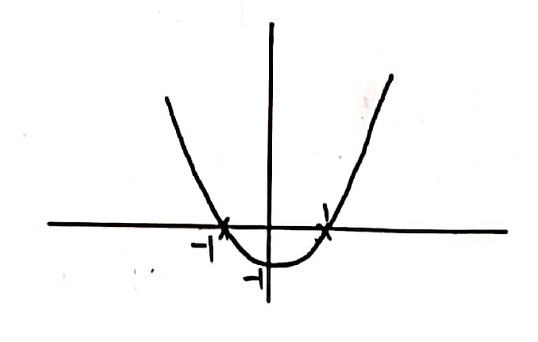
\includegraphics[width=1.8in,height=1.8in]{figures/ch08/figure1111_6.png}
	%\caption{This is an inserted JPG graphic} 
	%\label{fig:graph} 
	\end{marginfigure}
\end{enumerate}

%Above are notes for Nov 11


%Below are notes for Nov 13

\begin{align*}
\min_x\quad & F_0(x) \\
s.t.\quad & F_i(x) \leq 0 \quad i = 1,...,m\\
& a_i^Tx - b_i = 0\quad i = 1,...,p
\end{align*}

\begin{itemize}
	\item $F_o, F_1,...,F_m$ are convex
	
	\item $Ax - b = 0$
\end{itemize}

\begin{definition}
	$x\in \mathcal{C}$ is local optimum for a constrained optimization if $\exists \epsilon > 0$, $s.t.\forall y\in \mathcal{C}$ and $\Vert x-y\Vert < \epsilon$, we have $F_0(y) \geq F_0(x)$
\end{definition}

\begin{theorem}
	For a convex optimization problem a local minimum is also a global optimum. 
\end{theorem}


We prove this theorem for two particular instances:
\begin{enumerate}
	\item Unconstrained optimization problem
	
	\item Differentiable objective function $F_0$
\end{enumerate}

\begin{proof}
    
    For the first instance, suppose $x\in \mathcal{C}$ is not globally optimal but is locally minimal.
	
	$\rightarrow$ Because not globally optimal, $\exists y\in \mathcal{C}$ s.t. $F_0(y)<F_0(x)$
	
	$\rightarrow$ Consider $z = \lambda x + (1-\lambda)y\in \mathcal{C}$, because $\mathcal{C}$ is convex, so we have
	\begin{align*}
	F_0(z) &\leq \lambda F_0(x) + (1-\lambda)F_0(x)\\
	&< \lambda F_0(x) + (1-\lambda)F_0(x)\\
	&= F_0(x)
	\end{align*}
	
	$\rightarrow$ By picking $\lambda$ sufficiently close to $1$ (but $< 1$), $z\in \mathcal{C}$ is in neighborhood of $x$ and has a lower cost, so $x$ cannot be local minimum, and thus lead to a contradiction.
	
	Hence, for a unconstrained convex optimization problem, a local minimum must also be global minimum.
	
	As for the case $F_0$ is differentiable and convex
	\begin{align*}
	\min_x\quad & F_0(x) \\
	s.t.\quad & F_i(x) \leq 0 \quad i = 1,...,m\\
	& a_i^Tx - b_i = 0\quad i = 1,...,p
	\end{align*}

	\begin{itemize}
	\item For unconstrained case $x^*$ is optimal iff $\nabla F(x^*) = 0$
	
	\item For constrained optimization it is very possible there is no $x\in \mathcal{C}$ satisfies $\nabla F(x) = 0$
	\end{itemize}

	Therefore, in this case a local minimum is also a global minimum(recall that first order condition is a necessary condition for a local optimum but not a sufficient condition).
	\end{proof}



\begin{theorem}
	For a convex optimization problem with (convex) feasible set $\mathcal{C}$ and differentiable (convex) objective $F_0: \reals^n \rightarrow \reals$, a point $x^* \in \mathcal{C}$ is optimal iff:
	\begin{equation*}
	\nabla F_0(x^*)^T(y - x^*) \geq 0  \quad \forall y \in \mathcal{C}
	\end{equation*}

That is, start at the point $x^*\in \mathcal{C}$, move into feasible set in direction $v$ and then evaluate $F_0(x^*+tv)$. $F_0(x^*+tv)$ must be non-decreasing for $t\geq 0$.
\end{theorem}

\begin{marginfigure}
\centering
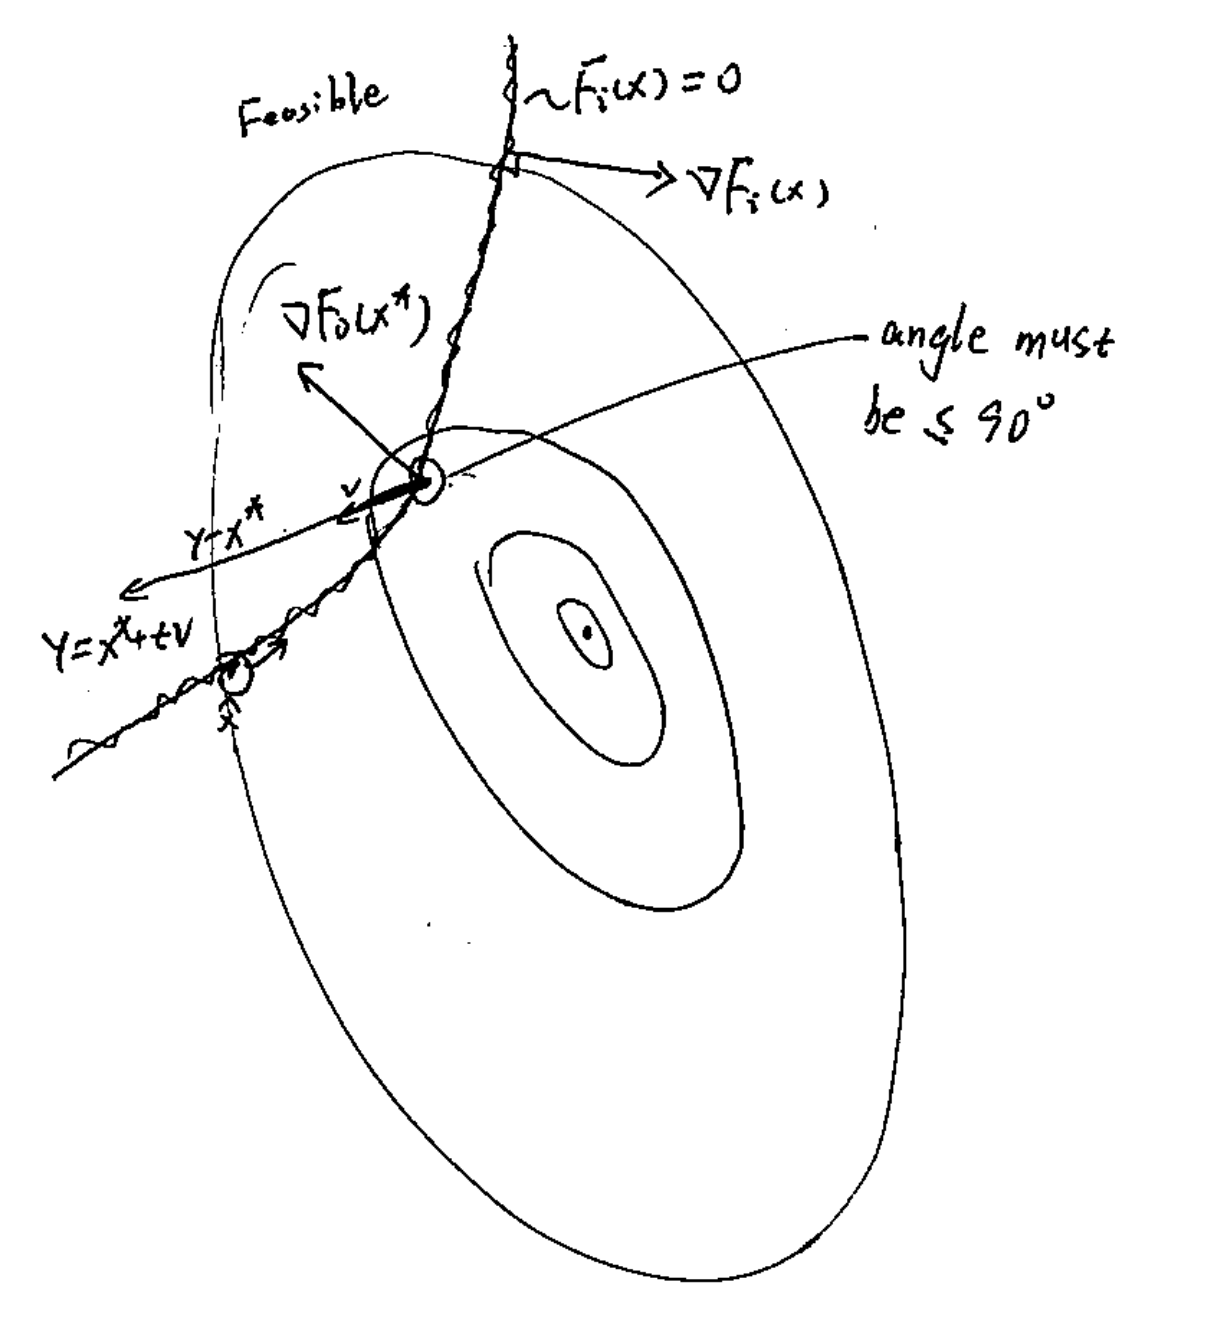
\includegraphics[width=1.8in,height=1.8in]{figures/ch09/figure1113_1.png}
%\caption{This is an inserted JPG graphic} 
%\label{fig:graph} 
\end{marginfigure}

\begin{proof}
	First assume the inequality holds, and we show that $x^*$ is the global optimum. A
	
	Apply $1$-st order condition for optimality, i.e. $\forall y \in \mathcal{C}$:
	\begin{align*}
	F_0(y) &\geq F_0(x^*) + \nabla F_0(x^*)^T(y-x^*)\\
	&\geq F_0(x^*)
	\end{align*}
	where the second term on the r.h.s. must be non-negative by our assumption.
	
	So for $\forall y \in \mathcal{C}$, we have $F_0(y)\geq F_0(x^*)$. Hence $x^*$ is a global optimum if the inequality holds.
	
	Secondly, we show that, if $x^*$ is the global optimum, then the inequality must holds. We prove this by contradiction.
	
	Suppose that $\exists y\in \mathcal{C}$ such that $\nabla F_0(x^*)^T(y-x^*)<0$.
	
	Look at the point $z$ defined as
	\begin{align*}
	z 
	&= \lambda y + (1-\lambda)x^*\\
	&= x^* + \lambda(y-x^*)
	\end{align*}
	
	All the points $z$ defined above must be feasible $\forall \lambda \in [0,1]$, because the set $\mathcal{C}$ is a convex set.
	
	We claim that, there exists some points $z$ such that $F_0(z)<F_0(x^*)$, by showing that
	\begin{align*}
	\left.\frac{dF_0(z)}{d\lambda}\right|_{\lambda = 0} &=\left.\frac{d}{d\lambda}F_0(x^*+\lambda(y-x^*))\right|_{\lambda = 0}\\
	&= \nabla F_0(x^*)^T(y-x^*)\\
	&< 0
	\end{align*}
	
	Since the slope(the gradient) is strictly negative(as we assume the inequality does not hold), the value of $F_0(z)$ will decreases as $\lambda>0$ increase, so we will have a smaller value $F_0(z)$ compared to $F_0(x^*)$, which contradicts the global optimality of $x^*$.
	
	Therefore, if the inequality does not hold, $x^*$ will not be the global optimum. So $x^*$ is the global optimum if and only if the inequality holds.
\end{proof}


\subsection{Quasi-convex minimization}
\begin{definition}
A function $F_0: \reals^n\to\reals$ is called quasi-convex if its domain and all
its sub-level sets are convex sets. 
\end{definition}

\begin{definition}
A function $F_0: \reals^n\to\reals$ is called quasi-concave if $-F_0$ is quasi-convex, that is, all its super-level sets are convex sets.
\end{definition}

\begin{definition}
If a function is both quasi-convex and quasi-concave, i.e., all its sub-level sets and super-levels are convex sets, then it is called quasi-linear.
\end{definition}

Consider the Quasi-convex minimization problem as follows,
\begin{align*}
\min_x\quad & F_0(x) \quad \text{quasi-convex}\\
s.t.\quad & F_i(x) \leq 0 \quad i = 1,\cdots,m\quad \text{convex}\\
& a_i^T - b_i = 0\quad i = 1,\cdots,m \quad \text{affine}
\end{align*}
We can rewrite this formulation into the form of feasibility problem,
\begin{align*}
\min_x\quad & \\%F_0(x) \quad \leftarrow \text{convex set}\\
s.t.\quad  & F_0(x) \leq t  \\
& F_i(x) \leq 0 \quad i = 1,\cdots,m \\
& a_i^T - b_i = 0\quad i = 1,\cdots,m
\end{align*}
where the constraint $F_0(x) \leq t$ defines a convex set(sub-level set is a convex set).

\begin{example}
	Consider the function $F_0(x) = \log x$ defined on $R_{++}$.
	
	We can show that, the sub-level sets of $F_0(x)$ are convex sets, so it is quasi-convex; the super-level sets of $F_0(x)$ are convex sets, so it is also quasi-concave. 
	
	Therefore, we call the function $F_0(x) = \log x$ is quasi-linear.
\end{example}



\begin{example}
	Consider the function $F_0(x) = \frac{P(x)}{Q(x)}$, where $P(x)$ is convex and non-negative(to make sure $t\geq 0$), $Q(x)$ is concave and $\text{dom}\ F_0 = \{x\vert Q(x) >0 \}$.
	
	So the sub-level set of this function can be expressed as
	\begin{align*}
	\{x\vert F_0(x) \leq t \} &= \{x\vert \frac{P(x)}{Q(x)}\leq t \}\\
	&= \{x\vert P(x)\leq tQ(x) \}\\
	&= \{x\vert P(x) - tQ(x)\leq 0 \}
	\end{align*}
	which is a convex set, since $P(x)$ and $-Q(x)$ are convex functions(so $P(x)-tQ(x)$ is convex as well), $t\geq 0$ and the set is the pre-image of a convex set under a convex function.
	
	Hence, the function $F_0(x) = \frac{P(x)}{Q(x)}$ is quasi-convex since all its sub-level sets are convex sets.
	
	Let's consider the special case for this kind of functions by setting $F_0(x)= \frac{a^T x+b}{c^T x +d}$ with $\text{dom}\ F_0=\{x\mid c^T x+d >0 \}$.
	
	We can show that(by similar approach above), the sub-level sets and super-level sets are convex sets, and thus $F_0(x)= \frac{a^T x+b}{c^T x +d}$ is quasi-linear(both quasi-convex and quasi-concave).

\end{example}

 Important note:
 
 (1) Quasi-convex optimization problems may have local optimum that are NOT global optimum (differ from the convex optimization problems).



\vspace{0.5cm}
\subsection{Convex optimization problem with generalized inequality constraints}
Convex optimization problem with generalized inequality constraints is an useful generalized version of convex optimization problem. By using the generalized inequalities in the constraints, the problem is formulated as
\begin{align*}
\min_x\quad & F_0(x) \\
s.t.\quad & F_i(x) \leq_{k_i} 0 \quad i = 1,...,m\\
& h_i(x) = 0\quad i = 1,...,m 
\end{align*}
where $F_0:\reals^n\to \reals$ is convex, $F_i: \reals^n\to \reals^l$ is "$k_i$-convex" and $k_i$ are cones. Recall a bit about the $k_i$-convex, which means $\forall \lambda\in [0, 1]$ we have
$$F_i(\lambda x + (1-\lambda)y)\leq_{k_i} \lambda F_i(x) + (1-\lambda)F_i(y)$$


Notice that, many of the results for ordinary convex optimization problems hold for problems with generalized inequalities. Some examples are:

(1) The feasible set, any sub-level set, and the optimal set are convex.

(2) Any point that is locally optimal for the problem is globally optimal.

(3) The optimality condition for differentiable $F_0$ in ordinary convex optimization problems still holds in this problem, without any change.


\vspace{0.3cm}
\subsection{Semi-definite program(SDP)}
When above cone $k$ is $S^n_+$, the cone of PSD $n$ by $n$ matrices, a special case of convex optimization problem with generalized inequality constraints is, the Semi-definite program(SDP) problem,
\begin{align*}
\min_x\quad & c^Tx \\
s.t.\quad & A_0+A_1x_1+\cdots+A_nx_n\leq 0\quad \\
& Fx = g
\end{align*}
where the inequality constraint is defined by a linear matrix inequity (LMI), $A_i\in S^n$, and $-(A_0+A_1x_1+\cdots+A_nx_n)\in S^n_+$. Note that here $\geq$ is understood as $\geq_k$, and thus for some symmetry matrices $Z\geq 0$ means that $Z$ is PSD. We will return to SDP later in this chapter and have more discussion.



%Above are notes for Nov 13





%Below are notes for Nov 18

\subsection{Second-Order Cone Program (SOCPs)}
A SOCP problem is formulated as
\begin{align*}
\min \quad&F^Tx\\
s.t. \quad& \Vert A_ix+b_i\Vert_2 \leq c_i^Tx + d_i\quad i = 1,...,m\\
&Fx \leq g
\end{align*}
where $A_i\in \reals^{n_i\times n}$, $x\in \reals^n$, $b_i\in \reals^{n_i}$, $F\in \reals^{p\times n}$ and $g\in \reals^p$.

Norm cone:
\begin{equation*}
\mathcal{C} = \{(x,t)\in \reals^{n+ 1} \vert \Vert x\Vert \leq t \} \subseteq \reals^{n+1}
\end{equation*}


\begin{marginfigure}
\centering
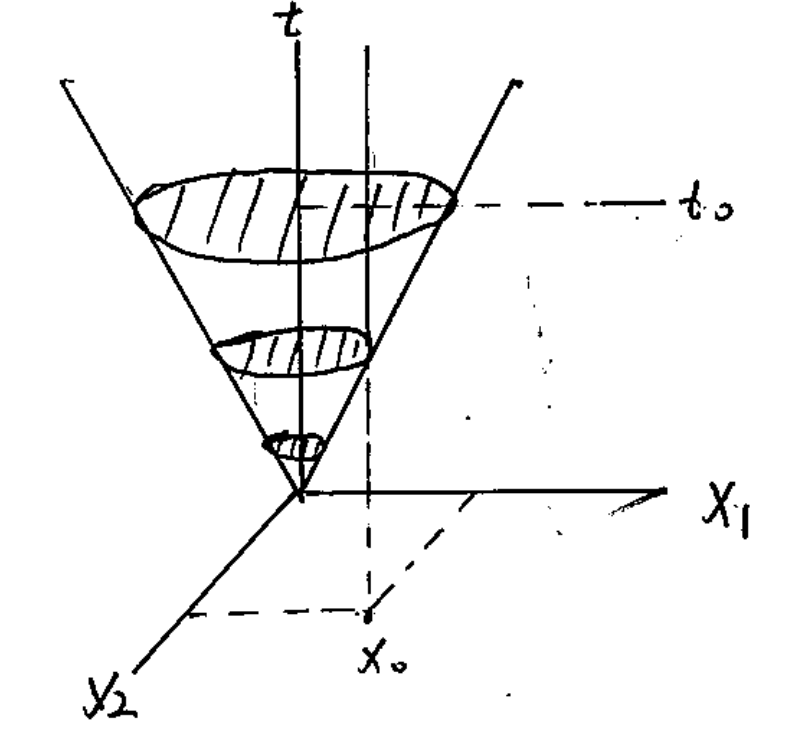
\includegraphics[width=1.8in,height=1.8in]{figures/ch09/figure1118_1.png}
%\caption{This is an inserted JPG graphic} 
%\label{fig:graph} 
\end{marginfigure}

\begin{itemize}
	\item First fix $t = t_0$, $\mathcal{C}_{t_0} = \{(x,t_0)\vert \Vert x\Vert \leq t_0 \}$, "fill-in" slice
	
	\item Next fix $x = x_0$, $\mathcal{C}_{x_0} = \{(x_0,t)\vert \Vert x_0\Vert \leq t \}$
	
	$\rightarrow$  Fix point in $x\in \reals^n$ to $x = x_0$ and "Fill up".
\end{itemize}


\begin{proof}
	We first prove that the set $\mathcal{C}$ is a Cone, and then prove it is a convex cone on the second part.
	
	\begin{enumerate}
		\item Pick any $(x_0, t_0)\in \mathcal{C}$, we show that for $(\theta x_0, \theta t_0)\in \mathcal{C}$ and $\forall \theta \in \reals_+$, we have
		$$\Vert \theta x_0\Vert = \vert \theta \vert \Vert x_0\Vert = \theta \Vert x_0\Vert \leq \theta t_0$$
		Therefore, $\mathcal{C}$ is a cone.
		
		\item Pick $(x_0, t_0)\in \mathcal{C}$ and $(y_0, s_0)\in \mathcal{C}$, we show that the point 
		$$(\theta x_0 + (1-\theta)y_0, \theta t_0 + (1-\theta)s_0)\in \mathcal{C},\ \forall 0\leq \theta \leq 1$$
		That is,
		\begin{align*}
		\Vert \theta x_0 + (1-\theta)y_0\Vert 
		&\leq \Vert \theta x_0\Vert + \Vert (1-\theta)y_0\Vert\\
		&= \vert \theta \vert \Vert x_0\Vert + \vert (1-\theta) \vert \Vert y_0\Vert\\
		&= \theta \Vert x_0\Vert +  (1-\theta)\Vert y_0\Vert\\
		&\leq \theta t_0 + (1-\theta)s_0
		\end{align*}
		Therefore the set $\mathcal{C} = \{(x,t)\vert \Vert x\Vert_2 \leq t \}$ is convex, and thus it is a convex cone.
		\end{enumerate}
		\end{proof}
		
		
		\begin{example}
		Consider following affine map:
		\begin{equation*}
		F_i(x) = \begin{bmatrix}
		A_ix+b_i\\
		c_i^Tx+d_i
		\end{bmatrix}\in \reals^{n+ 1}
		\end{equation*}
		For $i$-th constraint, we want to have $\Vert A_ix+b_i\Vert \leq c^T_ix+d_i$, and this is equivalent to require
		\begin{equation*}
		\{x\vert F_i(x)\in \mathcal{C}_{n+ 1}\} = F_i^{-1}(\mathcal{C}_{n+ 1})
		\end{equation*}

		Remarks:
		\begin{enumerate}
		\item If all $A_i = 0$, then we get an general LP;
	
		\item If $c_i = 0$, then we get a QCQP (which is obtained by squaring each of the constraints);
	
		\item The constraint is a second-order cone constraint, since we  use $l_2$ norm for this cone.
		\end{enumerate}
		\end{example}



\subsection{Robust Linear Programs}
We consider a linear program in inequality form,
\begin{align*}
\min \quad&c^Tx\\
s.t. \quad&a_i^Tx\leq b_i\quad i = 1,\cdots,m
\end{align*}
in which there is some uncertainty or variation in the parameters $c$, $a_i$, $b_i$. To simplify the exposition we assume that $c$ and $b_i$ are fixed, and that $a_i$ are the parameters with uncertainty.

There are two versions for the robustness of uncertainty in $a_i$, that is, (1) worst-case  (2)statistical approach

\vspace{0.3cm}
(1) Worst Case: Assume $a_i$ are known to lie in given ellipsoids.

In this case, we know that 
$$a_i\in \xi_i = \{a\vert a = \bar{a_i} + P_iu, \Vert u \Vert \leq 1 \} $$
 where $P_i\in\reals^{n\times n}$ (If $P_i$ is singular we obtain ‘flat’ ellipsoids, of dimension rank $P_i$;
$P_i = 0$ means that $a_i$ is known perfectly).

Hence, the robust linear program problem is formulated as
\begin{align*}
\min\quad &c^Tx\\
s.t. \quad&a_i^Tx\leq b_i\quad \forall a_i \in \xi_i \quad i = 1,\cdots,m
\end{align*}

Notice that the constraint of above formulation can be expressed as
$$(\bar{a_i} + P_iu)^Tx\leq b_i\ \text{and}\ \Vert u_i\Vert \leq 1,\ \forall i = 1,\cdots,m$$
Or equivalently,
$$\sup_{\Vert u_i\Vert \leq 1}(\bar{a_i} + P_iu)^Tx\leq b_i,\ \forall i = 1,\cdots,m$$
Furthermore, this constraint can be expressed as a second order cone constraint, since
\begin{align*}
(\bar{a_i} + P_iu)^Tx &= \bar{a_i}^Tx + u^TP_i^Tx \\
&\leq \bar{a_i}^Tx + (\frac{P_i^Tx}{\Vert P_i^Tx\Vert})^TP_i^Tx\\
&= \bar{a_i}^Tx + \frac{x^TP_iP_i^Tx}{\Vert P_i^Tx\Vert_2}\\
&= \bar{a_i}^Tx + \Vert P_i^Tx\Vert_2
\end{align*}\\
so this robust LP can be expressed as the SOCP formulated as
\begin{align*}
\min\quad &c^Tx\\
s.t. \quad&\bar{a_i}^T + \Vert P_i^T x\Vert_2\leq b_i,\ \forall i = 1,\cdots,m
\end{align*}
Note that the additional norm terms act as regularization terms; they prevent $x$ from being large in directions with considerable uncertainty in the parameters $a_i$.


\vspace{0.3cm}
(2) Statistical approach: Assume that $a_i$ are independent Gaussian random vectors.

In this case, we assume that $a_i$ are independent Gaussian random vectors such that $a_i \sim N(\bar{a_i}, \Sigma_i)$.

Recall a little bit regarding the statistics, since each component $a_i$ are independent, we could consider the mean and variance for the random variables $a_i^Tx - b_i$ respectively,

The mean is given by
$$\mathbb{E}[a_i^Tx - b_i] = \bar{a_i}^Tx - b_i = \mu_i$$

The variance is given by
\begin{align*}
\mathbb{E}[((a_i^Tx - b_i) - (\bar{a_i}^Tx - b_i))^2] 
&= \mathbb{E}[((a_i - \bar{a_i})^Tx)^2]\\
&= \mathbb{E}[x^T(a_i - \bar{a_i})(a_i - \bar{a_i})^Tx] \\
&= x^T\mathbb{E}[(a_i - \bar{a_i})(a_i - \bar{a_i})^T]x\\
&= x^T\Sigma_i x \\
&= \sigma^2\\
&= x^T \Sigma_i^{\frac{1}{2}}\Sigma_i^{\frac{1}{2}} x\\
&= \Vert \Sigma_i^{\frac{1}{2}} x\Vert^2_2
\end{align*}

Since the constraints involve randomness, we would like to consider the probability such that the constraint holds, which is given by
\begin{align*}
\mathbb{P}[a^T_i x\leq b_i]
&= \Phi\left(\frac{b_i - \bar{a_i}^Tx}{\sigma_i}\right)\\
&= \Phi\left(\frac{b_i - \bar{a_i}^Tx}{\Vert \Sigma_i^{\frac{1}{2}} x\Vert_2}\right)
\end{align*}

\begin{marginfigure}
\centering
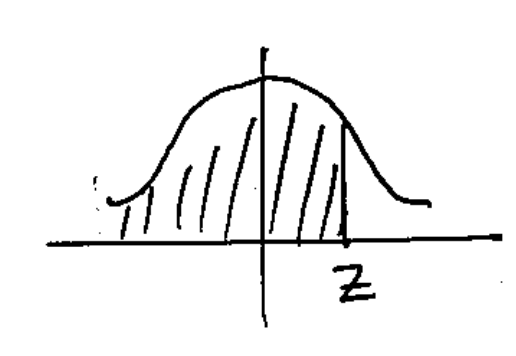
\includegraphics[width=1.8in,height=1.8in]{figures/ch09/figure1118_2.png}
%\caption{This is an inserted JPG graphic} 
%\label{fig:graph} 
\end{marginfigure}

Suppose now we require that each constraint should hold with a probability exceeding $\eta$, that is,
\begin{align*}
& \mathbb{P}[a_i^Tx\leq b_i]\geq \eta\\
\Leftrightarrow&\Phi(\frac{b_i - \bar{a_i}^Tx}{\sigma_i})\geq \eta\\
\Leftrightarrow&\frac{b_i - \bar{a_i}^Tx}{\sigma_i}\geq \Phi^{-1}(\eta)
\end{align*}

By above argument, we have the problem formulated as 
\begin{align*}
\min \quad& c^Tx \\
s.t. \quad& \mathbb{P}[a_i^Tx\leq b_i]\geq \eta,\ \forall i = 1,\cdots,m
\end{align*}
and it turns out(we have showed this fact above) that, this is equivalent to a SOCP problem as the following
\begin{align*}
\min \quad& c^Tx \\
s.t. \quad& b_i - \bar{a_i}^Tx\geq \Phi^{-1}(\eta)\Vert\Sigma_i^{\frac{1}{2}}x\Vert_2,\ \forall i = 1,\cdots,m
\end{align*}




\vspace{0.5cm}
\subsection{Geometric Program(GP)}
Before introducing GP, we give some definitions first,
\begin{itemize}
	\item "Monomial": $h(x) = cx_1^{\alpha_1}x_2^{\alpha_2}...x_n^{\alpha_n}$, $c>0, \alpha_i\in \reals$, $\text{dom} h = (x\vert x_i>0 \quad \forall i\in {1...n})$
	
	\item Posynomial: $F(x) = \sum^k_{k=1}c_kx_1^{\alpha_{1k}}x_2^{\alpha_{2k}}...x_n^{\alpha_{nk}}$(sum of monomials)
	
	$\rightarrow$ note closed under addition, multiplication, non-negative scaling.
\end{itemize}

With these definitions in mind, a Geometric program problem is formulated as 
\begin{align*}
\min\quad &F_0(x)\\
s.t. \quad&F_i(x)\leq 1,\quad i = 1,\cdots,m\\
&h_i(x)= 1,\quad i = 1,\cdots,p
\end{align*}
where $x\in\reals^{n}$, $F_0, F_1,\cdots,F_m$ are posynomials, $h_0, h_1,\cdots,h_m$ are monomials. 


Geometric programs are not (in general) convex optimization problems, but they can be transformed to convex problems by a change of variables and a transformation of the objective and constraint functions.

To get a GP into convex form, we set $y_i = log x_i$, so $x_i = e^{y_i}$ (recall $x_i > 0$). Hence, we have

Transformation of monomials:
\begin{align*}
&h(x_1,x_2,\cdots,x_m) = cx_1^{\alpha_1}x_2^{\alpha_2}\cdots x_n^{\alpha_n}\\
\Leftrightarrow& \log h(x_1,x_2,\cdots,x_m) = \log c + \alpha_1 \log x_1 +\alpha_2 \log x_2 + \cdots + \alpha_n \log x_n\\
\Leftrightarrow& \log h(e^{y_1},e^{y_2},\cdots,e^{y_m}) = \log c + \alpha_1 y_1 +\alpha_2 y_2 + \cdots + \alpha_n y_n
\end{align*}
and this an affine function of $y_i$, and thus it is convex.

Transformation of posynomials:
\begin{align*}
&F(x_1,\cdots,x_n) = \sum^k_{i=1}c_kx_1^{\alpha_{1k}}x_2^{\alpha_{2k}}\cdots x_n^{\alpha_{nk}}\\
\Leftrightarrow& \log F(e^{y_1},e^{y_2},\cdots,e^{y_n}) = \log(\sum^k_{k=1}e^{\log c_k}e^{\alpha_{1k}y_1}\cdots e^{\alpha_{nk}y_n})\\
\Leftrightarrow& \log F(e^{y_1},e^{y_2},\cdots,e^{y_n})             =\log(\sum^k_{k=1}e^{\alpha_{1k}y_1+\cdots+\alpha_{nk}y_n+\log c_k})
\end{align*}
and we could show this is also a convex function of $y_i$.

With above transformations, we have the geometric program in convex form, 
\begin{align*}
\min\quad & \log F_0(e^{y_1},e^{y_2},\cdots,e^{y_n}) \\
s.t. \quad& \log F_i(e^{y_1},e^{y_2},\cdots,e^{y_n}) \leq \log(1) = 0,\ \forall i=1,\cdots,m\\
&\log h_i(e^{y_1},e^{y_2},\cdots,e^{y_n}) = 0,\ \forall i=1,\cdots,q
\end{align*}

Note that:

(1) To distinguish the GP from the original formulation and this convex one, we refer to the original as a geometric program in posynomial form, and the one after transformation as the geometric program in convex form.

(2) If the posynomial objective and constraint functions all have only one term, i.e., are monomials, then the convex form geometric program reduces to a (general) linear program.


%Below are notes for Nov 20
\vspace{0.5cm}
\subsection{Semi-definite Programs(SDPs)}
Recall that, a SDP is formulated as 
\begin{align*}
\min \quad&c^Tx \\
s.t. \quad&F_0 + x_1F_1 + x_2F_2 + ... + x_nF_n \leq 0\\
&Gx = h
\end{align*}
where $F_0, F_1, \cdots, F_n \in S^m$, and inequality constraint here is a linear matrix inequality.

We show that, the inequality constraint above indeed defines a convex set, and more precisely, is a PSD cone. Since
\begin{equation*}
F(x) := F_0 + x_1F_1 + x_2F_2 + \cdots + x_nF_n  \leq 0 \Leftrightarrow -F(x) \geq 0
\end{equation*}
so $ -F(x) \in S_+^m$, and thus $\{x\vert -F(x)\in S^n_+ \}$ is a convex set. 

Alternatively, we could also consider the standard form of a SDP:
\begin{align*}
\min \quad&\trace(CZ) \\
s.t. \quad&\trace(A_iZ) = b_i, \quad i = 1, \cdots, m\\
&Z\geq 0
\end{align*}

To obtain the above standard form, similar with what we did in LP, we

(1) Introduce slack variables(variables that are non-negative) into inequality constraints and then obtain equality constraints;
	
(2) Decompose $x_i$ by $x_i = x_i^+ - x_i^-$, $x_i^+\geq 0$, $x_i^-\geq 0$.


\vspace{0.5cm}
\subsection{Relaxation of homogeneous QCQP}
First, recall that a QCQP problem is formulated as 
\begin{align*}
\min \quad&\frac{1}{2}x^TP_0x + q_0^Tx + r_0 \\
s.t. \quad&\frac{1}{2}x^TP_ix + q_i^Tx + r_i\leq 0,\quad i = 1,...,m\\
&Fx = g
\end{align*}

Notice that,
\begin{itemize}
	\item The QCQP is homogeneous if $q_i = 0, \forall i\in \{0,1,...m \}$;
	
	\item The QCQP is convex if all $P_i$ are PSD;
	
	\item The QCQP is non-convex if some $P_i$ are not PSD, or if we replace the inequality with a equality.
	
\end{itemize}

\vspace{0.3cm}
Now, lets consider the homogeneous QCQP with the following formulation
\begin{align*}
\min \quad&x^TCx \\
s.t. \quad&x^TF_ix \leq g_i\\
&x^TH_ix = l_i
\end{align*}
which is not necessary to be convex optimization problem.

Notice that
\begin{equation*}
x^TCx = \trace(x^TCx) = \trace(Cxx^T) = \trace(CX)
\end{equation*}
where we let $X := xx^T$, $\rank(X) = 1$, $X\geq0$. 

So, the above homogeneous QCQP can also be written as:
\begin{align*}
\min \quad&\trace(CX) \\
s.t. \quad&\trace(F_iX) \leq g_i, \quad i = 1,\cdots,m\\
&\trace(H_iX) = l_i, \quad i = 1,\cdots,p\\
&\rank(X) = 1\\
&X\geq 0
\end{align*}

Relaxation: Drop a constraint that is hard to deal with and thus we could solve an easier problem. 

$\rightarrow$ $\min$ is the lower bound to original problem's optimum value. 

$\rightarrow$ Maybe (if relaxation is good) you can figure out an $X$ that is a good enough solution to original:
\begin{equation*}
X^*_{relaxed} =\sum^n_{i=1}v_iv^T_i\lambda_i \Rightarrow \lambda_1v_1 v^T_1
\end{equation*}




\begin{example}{Two-way partitioning problem}
	
	Suppose now we have $n$ items, and we want to partition these $n$ items into 2 different sets while minimizing the total cost of the whole partition procedure. We let $x\in\reals^n$ be a partition for these $n$ items, in particular, each $x_i=1 \text{or} -1$ for $i=1,\cdots, n$, where $1$ and $-1$ represent 2 different sets.
	
	Let $W_{ij}$ be the cost of placing the items $i$ and $j$ in the same set, and $-W_{ij}$ be the cost of having $i$ and $j$ in different sets. So we define a matrix $W$ that contains these cost.
	
	\begin{marginfigure}
	\centering
	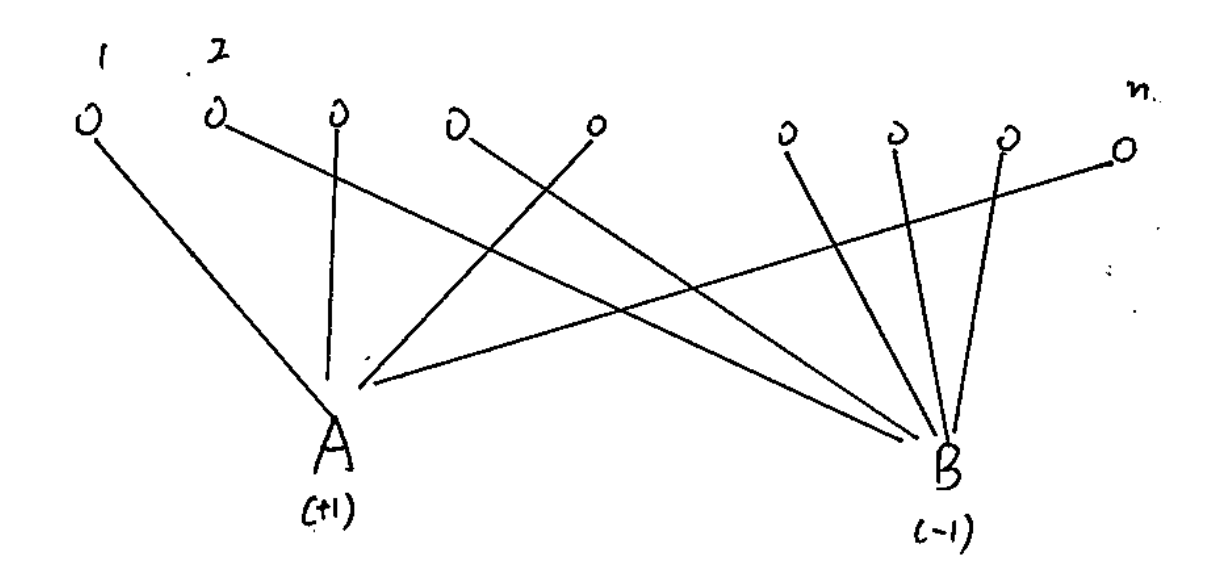
\includegraphics[width=1.8in,height=1.8in]{figures/ch09/figure1120_1.png}
	%\caption{This is an inserted JPG graphic} 
	%\label{fig:graph} 
	\end{marginfigure}

With this problem setting, this question can be formulated as a non convex optimization problem as follows
\begin{align*}
\min \quad&x^TWx \\
s.t. \quad&x_i\in \{1,-1 \},\ \forall i=1,\cdots, n
\end{align*}
Equivalently, we have
\begin{align*}
\min \quad&x^TWx \\
s.t. \quad&x_i^2 = 1,\ \forall i = 1,\cdots,n
\end{align*}

Notice that
\begin{equation*}
x^TWx = \sum^n_{i=1}W_{ii}(x_i)^2+\sum_{i\neq j}(W_{ij}+W_{ji})x_ix_j
\end{equation*}
and thus the original formulation can be expressed as
\begin{align*}
\min \quad&\trace(WX) \\
s.t. \quad&X_{ii} = 1,\ i = 1,\cdots,n\\
&X\geq 0\\
&\rank(X) = 1
\end{align*}
By relaxation, we drop the constraint $\rank(X) = 1$ so that we have a SDP problem.


\end{example}
%Above are notes for Nov 20
